%
%  Title       :  Requirements and Analysis Document
%  Authors     :  Alex Gerdes
%  Created     :  August 20, 2018
%
%  Purpose     :  Tempate RAD for TDA367/DIT212
%
%-------------------------------------------------------------------------------

\documentclass[12pt,a4paper]{scrartcl}

\usepackage[hyphens]{url}
\usepackage{hyperref}
\usepackage{xcolor}
\usepackage{graphicx}
\usepackage{mathpazo}
\usepackage{titling}
\usepackage{enumitem}
\renewcommand\maketitlehooka{\null\mbox{}\vfill}
\renewcommand\maketitlehookd{\vfill\null}


\title{Requirements and Analysis Document for }
\author{
\includegraphics[width=\textwidth]{paintit.png} }
\date{Henrik Lagergren, Markus Pettersson, Aron Sj\"oberg, \\ Ellen Widerstrand, Robert Zetterlund \\ 2/10/18\\v.1.0}


\begin{document}

\maketitle
\thispagestyle{empty}

\newpage
\thispagestyle{empty}
\tableofcontents{}


\newpage

\section{Introduction}
Here it should be some kind of major introduction

\setcounter{page}{1}

%Have you ever felt the urge to do something fun and exciting? Maybe felt an eager to share your creativity with the world? Then we have the solution for you and it´s called PaintIT.

%The project aims to create a desktop version of the popular mobile game paint Something developed by OMGPop. Even in 2018 not everyone has access to a smartphone nor internet connection. This is especially true in developing countries such as South Africa, and by making the application offline-compatible(?) PaintIT strives to be as accessible as possible to a broader demographic than ever before (!!!). The game is simple enough, two players take turn painting a given word and guessing what’s being depicted. It´s fun, exciting and suitable for all ages.

%The game is turn based.
%There are 2 players.
%The players take turns painting and guessing
%The goal is to guess as many correct words in a row as possible.
%There are no time constraints.
%The player that paints is given a word to depict.


\subsection{Purpose of application}
The project aims to create a desktop version of the popular mobile painting-game "paintSomething" developed by OMGPop. By using the desktop the user is able to use their mouse and their keyboard which allows for a smoother painting experience, further expanding on the simplistic and elegant mobile version. While catering for the advanced user, for example by using keyboard-shortcuts, PaintIt is also easy to play for the most inexperienced computer-user since it uses UI-design patterns (To read more read appendix section 1). 

Further, the applications aims to cater to children of developing countries. By being a member of the education-gaming genre the player will practice basic English words and express themselves artistically while simultaneously having fun.
\subsection{General characteristics of application}

The game is collaborative, meaning the users work together gaining points which is stored in a "streak" that is viewable in the highscore.
When starting the game, one of the users (from now on referred to as the guesser) is advised to look away whilst the other player is presented with a word, (from now on referred to as the painter). The painter's task is to paint the presented word with enough accuracy that the guesser will be able to guess the word using a set amount of tiles containing letters.. 


The application is an offline desktop game, %which follows the target groups prerequisites, 
users will gather to one computer and take turns painting and guessing. The game is originally designed to consist of two users, however, it is possible to paint and guess as a group, meaning the game can be played by virtually any amount of players.

\subsection{Scope of application}
The scope of the application lies within the hands of the player, meaning the experience is determined by the painter and the given word. What this effectively results in is a game where players rely on each other for a pleasant experience. The Game revolves around a basic loop, (more throughout explanation in the section below): 
\begin{enumerate}
    \item Receiving word
    \item Painting word
    \item Guessing word
\end{enumerate}

\subsection{Objectives and success criteria of the project}
\begin{enumerate}
	\item The game should save the team's streak and add it to the high score.
	\item Before starting the game, the players should be able to view the high score.
	\item It should be possible for the players to choose their names.
	\item Before the players begin to play, it should be possible to get information about how the game works and what they are supposed to do.
	\item One player, the painter, should get a word to paint, as well as a painting brush and canvas that he or she can use to paint the word. The other player, the guesser, should be able to see the painter's painting when it is finished and get letters that he or she can use to guess what the painter has painted. 
\end{enumerate}

\subsection{Definitions, acronyms, and abbreviations}
Below follows words that are used throughout the working process.
\subsubsection{General words used throughout document and development}
\begin{itemize}
    \item MVC - Model View Controller.
    \item JavaFX - The standard GUI library for Java. 
    \item UI - User Interface.
    \item Design Pattern - 
\end{itemize}

\subsubsection{Words explaining the game}
\begin{itemize}  
    \item \textbf{Painter} The player that is being presented a word and that is supposed to paint on the Canvas.
    
    \item \textbf{Word} The word that is supposed to be painted and guessed. 
    
    \item \textbf{Canvas} The canvas contains the painting of the painter, the canvas is also shown to the guesser.  

    \item \textbf{Guesser} The player that is being presented with a painting and eight tiles.
    
    \item \textbf{Tiles} A tile consists of 1 (one) letter, in total there are 8 (eight) tiles that has n amount of letters being of the words, (where n is and int of the amount of letters in a word)
    
    \item \textbf{Round} - A round consists of a word being presented, painted and guessed, either incorrectly or correctly.
    
    \item \textbf{Streak} - The amount of successful rounds, meaning the painting was guessed correctly. 
    
\end{itemize}
\subsubsection{Implementation definitions}   
\begin{itemize}
    \item \textbf{TopController} - Is a controller that shows and prepares views, unlike every other controller, it does not hold one (1) view, it holds all the views in the application within a list.

    \item \textbf{Canvas} - Not an actual class. The canvas is the umbrella term for the area which you can paint on. The Canvas consists of the CanvasModel, CanvasController and the CanvasView. 

    \begin{itemize}
         \item \textbf{CanvasModel} - The actual representation of the canvas. The CanvasModel consists of a 2D matrix of type Color. The model is observed by the CanvasView.
         \item \textbf{CanvasController} - The CanvasController recieves coordinates from the user via the CanvasView, and changes the model accordingly with regards to the equipped Tool.
        \item \textbf{CanvasView} - The actual view of the canvas, it extends the JavaFX Class Canvas and uses a pixelWriter to change pixels.
    \end{itemize} 

    \item \textbf{Tool} - \Huge{[REDACTED]} \small Currently an interface which is implemented by Brush, SprayCan, Eraser. Tools is observed by CanvasController and calls the update(int x, int y, Color color).
    
    \begin{itemize}
        \item \textbf{Brush} -
        \item \textbf{SprayCan} -
        \item \textbf{Eraser} -
    \end{itemize}

\end{itemize}

\newpage
\section{Requirements}
Below follows requirements.
\subsection{Functional Requirements}
The players should be able to:
\begin{enumerate}

    \item Navigate around the main menu.

    \begin{enumerate}[label=\alph*.]
        \item Be able to read the rules.
        \item Look at the highscore
        \item Go to the game setup screen.
            \begin{enumerate}[label=\roman*.]
                \item Choose the player names
                \item Choose playstyle
                \item Choose timelimit.
                \item Choose difficulty.
            \end{enumerate}
    \end{enumerate}
    
    \item Play the game.
    \begin{enumerate}[label=\alph*.]
        \item The Painter should be able to:
        \begin{enumerate}[label=\alph*.]
            \item Paint on the canvas using the
                 \begin{enumerate}[label=\roman*.]
                    \item Brush
                    \item SprayCan
                    \item Eraser
                 \end{enumerate}
            \item Choosing color to paint with.
            \item Choosing the radius to paint with.
            \item Clear the entire canvas.
            \item Undo the latest stroke of paint.
        \end{enumerate}
        \item The Guesser should be able to:
        \begin{enumerate}[label=\alph*.]
            \item See the painted canvas.
            \item See a selection of eight tiles.     
            \item See an empty word sequence.
            \item Guess the word by:
                 \begin{enumerate}[label=\roman*.]
                    \item Moving the given tiles to the word sequence.
                    \item Removing tiles from word sequence.
                    \item Asking for hints.
                 \end{enumerate}
            \item Give up.
        \end{enumerate}
        \item At the end of the round select to start a new round or end game session.
    \end{enumerate}
    \item Exit the application and store game-streak.
\end{enumerate}

The application should be able to:
\begin{enumerate}
    \item ...?
\end{enumerate}

\subsection{Non-functional Requirements}
Below follows something about something.
\subsubsection{Usability}
Playing the game requires basic computer knowledge, primarily usage of the mouse to navigate the application and to paint. Further, some experience with drawing programs, msPaint for example, would be beneficial since similar techniques are used throughout the painting process. The program adjusts for different levels of knowledge within the English language, however some English knowledge is required. 
\subsubsection{Reliability}
//not applicable//
\subsubsection{Performance}
The application should not have any delay on a regular computer, except when using the undo and clear functionality while painting. These two buttons redraws a large portion of the canvas, while storing the change, meaning a lot of computer processing power.
\subsubsection{Supportability}
The application is developed to work on Windows, Mac and Linux platforms. The application is able to be expanded to online-play, however, due to time constraints it was determined not necessary. 
\subsubsection{Implementation}
The application is written in Java and uses the standard library JavaFX for the GUI.
\subsubsection{Packaging and installation}
To run the program you will need to be able to execute a .jar file.
\subsubsection{Legal}

\subsection{User Stories}
Use the template from the course website and list all user stories here. It is
fine to have them in an spreadsheet (or other application) at first, but they 
must end up here as well.

These user stories should describe what the user will be able to do. Write a 
the user stories in language of the customer, and give the a unique ID. List the
user stories in priority order.

\subsection{User interface}

Sketches, paintings and explanations of the application user interface (possible
navigation).


\section{Domain model}

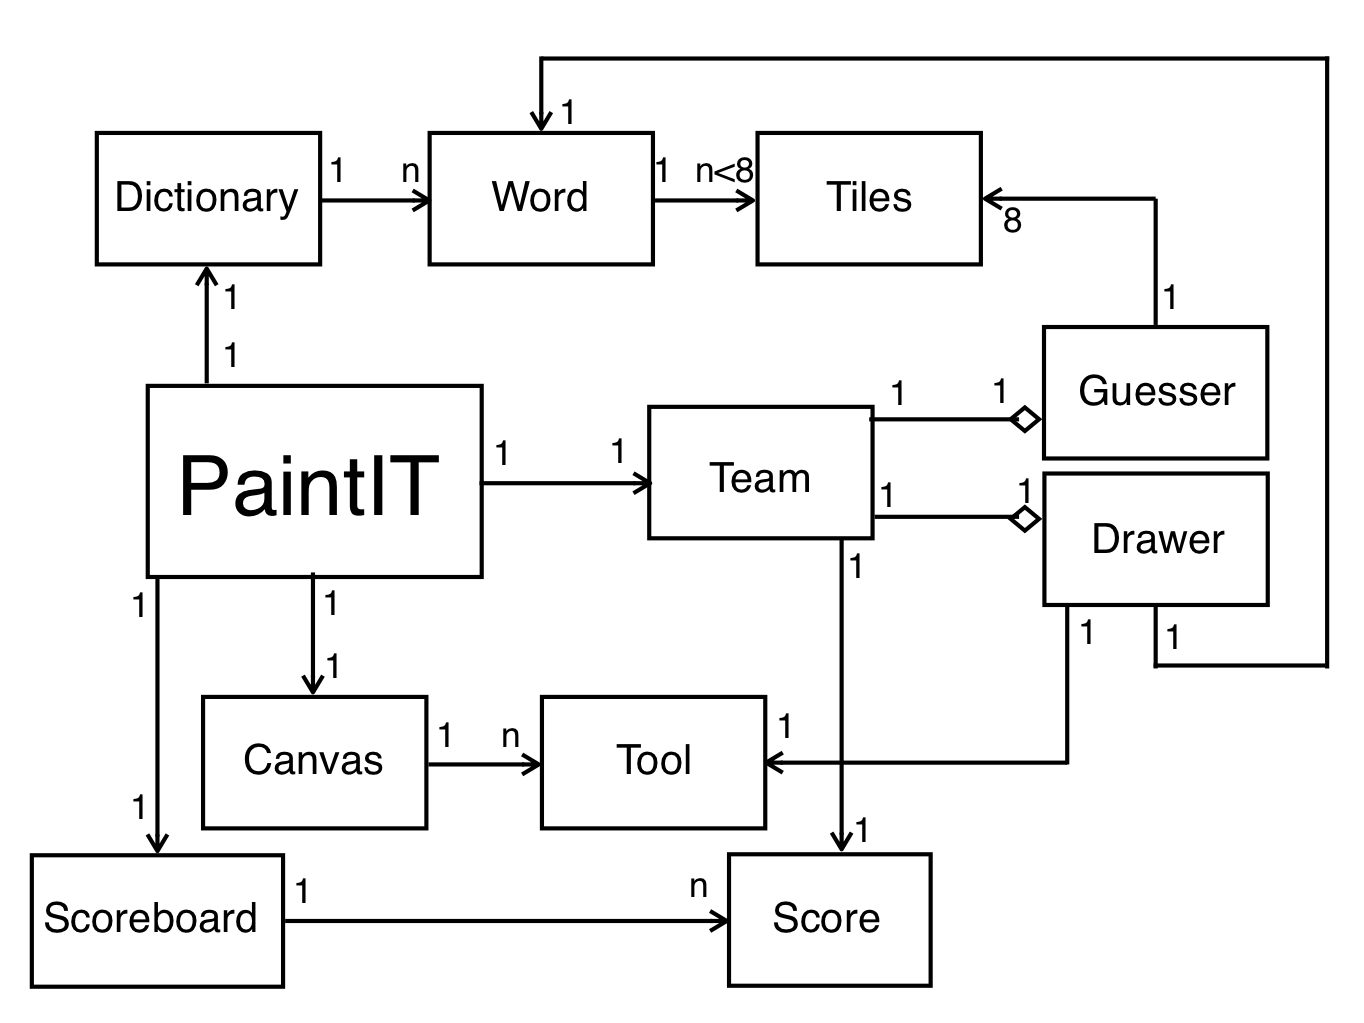
\includegraphics[width=\textwidth]{domainModel.png}

\subsection{Class responsibilities}

Explanation of responsibilities of classes in diagram.


\section{References}


\end{document}
